% This is the Reed College LaTeX thesis template. Most of the work
% for the document class was done by Sam Noble (SN), as well as this
% template. Later comments etc. by Ben Salzberg (BTS). Additional
% restructuring and APA support by Jess Youngberg (JY).
% Your comments and suggestions are more than welcome; please email
% them to cus@reed.edu
%
% See https://www.reed.edu/cis/help/LaTeX/index.html for help. There are a
% great bunch of help pages there, with notes on
% getting started, bibtex, etc. Go there and read it if you're not
% already familiar with LaTeX.
%
% Any line that starts with a percent symbol is a comment.
% They won't show up in the document, and are useful for notes
% to yourself and explaining commands.
% Commenting also removes a line from the document;
% very handy for troubleshooting problems. -BTS

% As far as I know, this follows the requirements laid out in
% the 2002-2003 Senior Handbook. Ask a librarian to check the
% document before binding. -SN

%%
%% Preamble
%%
% \documentclass{<something>} must begin each LaTeX document
\documentclass[12pt,twoside]{reedthesis}
% Packages are extensions to the basic LaTeX functions. Whatever you
% want to typeset, there is probably a package out there for it.
% Chemistry (chemtex), screenplays, you name it.
% Check out CTAN to see: https://www.ctan.org/
%%
\usepackage{graphicx,latexsym}
\usepackage{amsmath}
\usepackage{amssymb,amsthm}
\usepackage{longtable,booktabs,setspace}
\usepackage{chemarr} %% Useful for one reaction arrow, useless if you're not a chem major
\usepackage[hyphens]{url}
% Added by CII
\usepackage{hyperref}
\usepackage{lmodern}
\usepackage{float}
\floatplacement{figure}{H}
% End of CII addition
\usepackage{rotating}

% Next line commented out by CII
%%% \usepackage{natbib}
% Comment out the natbib line above and uncomment the following two lines to use the new
% biblatex-chicago style, for Chicago A. Also make some changes at the end where the
% bibliography is included.
%\usepackage{biblatex-chicago}
%\bibliography{thesis}


% Added by CII (Thanks, Hadley!)
% Use ref for internal links
\renewcommand{\hyperref}[2][???]{\autoref{#1}}
\def\chapterautorefname{Chapter}
\def\sectionautorefname{Section}
\def\subsectionautorefname{Subsection}
% End of CII addition

% Added by CII
\usepackage{caption}
\captionsetup{width=5in}
% End of CII addition

% \usepackage{times} % other fonts are available like times, bookman, charter, palatino

% Syntax highlighting #22
  \usepackage{color}
  \usepackage{fancyvrb}
  \newcommand{\VerbBar}{|}
  \newcommand{\VERB}{\Verb[commandchars=\\\{\}]}
  \DefineVerbatimEnvironment{Highlighting}{Verbatim}{commandchars=\\\{\}}
  % Add ',fontsize=\small' for more characters per line
  \usepackage{framed}
  \definecolor{shadecolor}{RGB}{248,248,248}
  \newenvironment{Shaded}{\begin{snugshade}}{\end{snugshade}}
  \newcommand{\AlertTok}[1]{\textcolor[rgb]{0.94,0.16,0.16}{#1}}
  \newcommand{\AnnotationTok}[1]{\textcolor[rgb]{0.56,0.35,0.01}{\textbf{\textit{#1}}}}
  \newcommand{\AttributeTok}[1]{\textcolor[rgb]{0.77,0.63,0.00}{#1}}
  \newcommand{\BaseNTok}[1]{\textcolor[rgb]{0.00,0.00,0.81}{#1}}
  \newcommand{\BuiltInTok}[1]{#1}
  \newcommand{\CharTok}[1]{\textcolor[rgb]{0.31,0.60,0.02}{#1}}
  \newcommand{\CommentTok}[1]{\textcolor[rgb]{0.56,0.35,0.01}{\textit{#1}}}
  \newcommand{\CommentVarTok}[1]{\textcolor[rgb]{0.56,0.35,0.01}{\textbf{\textit{#1}}}}
  \newcommand{\ConstantTok}[1]{\textcolor[rgb]{0.00,0.00,0.00}{#1}}
  \newcommand{\ControlFlowTok}[1]{\textcolor[rgb]{0.13,0.29,0.53}{\textbf{#1}}}
  \newcommand{\DataTypeTok}[1]{\textcolor[rgb]{0.13,0.29,0.53}{#1}}
  \newcommand{\DecValTok}[1]{\textcolor[rgb]{0.00,0.00,0.81}{#1}}
  \newcommand{\DocumentationTok}[1]{\textcolor[rgb]{0.56,0.35,0.01}{\textbf{\textit{#1}}}}
  \newcommand{\ErrorTok}[1]{\textcolor[rgb]{0.64,0.00,0.00}{\textbf{#1}}}
  \newcommand{\ExtensionTok}[1]{#1}
  \newcommand{\FloatTok}[1]{\textcolor[rgb]{0.00,0.00,0.81}{#1}}
  \newcommand{\FunctionTok}[1]{\textcolor[rgb]{0.00,0.00,0.00}{#1}}
  \newcommand{\ImportTok}[1]{#1}
  \newcommand{\InformationTok}[1]{\textcolor[rgb]{0.56,0.35,0.01}{\textbf{\textit{#1}}}}
  \newcommand{\KeywordTok}[1]{\textcolor[rgb]{0.13,0.29,0.53}{\textbf{#1}}}
  \newcommand{\NormalTok}[1]{#1}
  \newcommand{\OperatorTok}[1]{\textcolor[rgb]{0.81,0.36,0.00}{\textbf{#1}}}
  \newcommand{\OtherTok}[1]{\textcolor[rgb]{0.56,0.35,0.01}{#1}}
  \newcommand{\PreprocessorTok}[1]{\textcolor[rgb]{0.56,0.35,0.01}{\textit{#1}}}
  \newcommand{\RegionMarkerTok}[1]{#1}
  \newcommand{\SpecialCharTok}[1]{\textcolor[rgb]{0.00,0.00,0.00}{#1}}
  \newcommand{\SpecialStringTok}[1]{\textcolor[rgb]{0.31,0.60,0.02}{#1}}
  \newcommand{\StringTok}[1]{\textcolor[rgb]{0.31,0.60,0.02}{#1}}
  \newcommand{\VariableTok}[1]{\textcolor[rgb]{0.00,0.00,0.00}{#1}}
  \newcommand{\VerbatimStringTok}[1]{\textcolor[rgb]{0.31,0.60,0.02}{#1}}
  \newcommand{\WarningTok}[1]{\textcolor[rgb]{0.56,0.35,0.01}{\textbf{\textit{#1}}}}

% To pass between YAML and LaTeX the dollar signs are added by CII
\title{Thesis}
\author{Sarah Maebius}
% The month and year that you submit your FINAL draft TO THE LIBRARY (May or December)
\date{December 6th, 2020}
\division{Mathematics and Natural Sciences}
\advisor{Tom Allen}
\institution{Reed College}
\degree{Bachelor of Arts}
%If you have two advisors for some reason, you can use the following
% Uncommented out by CII
% End of CII addition

%%% Remember to use the correct department!
\department{Mathematics}
% if you're writing a thesis in an interdisciplinary major,
% uncomment the line below and change the text as appropriate.
% check the Senior Handbook if unsure.
%\thedivisionof{The Established Interdisciplinary Committee for}
% if you want the approval page to say "Approved for the Committee",
% uncomment the next line
%\approvedforthe{Committee}

% Added by CII
%%% Copied from knitr
%% maxwidth is the original width if it's less than linewidth
%% otherwise use linewidth (to make sure the graphics do not exceed the margin)
\makeatletter
\def\maxwidth{ %
  \ifdim\Gin@nat@width>\linewidth
    \linewidth
  \else
    \Gin@nat@width
  \fi
}
\makeatother

%Added by @MyKo101, code provided by @GerbrichFerdinands

\renewcommand{\contentsname}{Table of Contents}
% End of CII addition

\setlength{\parskip}{0pt}

% Added by CII

\providecommand{\tightlist}{%
  \setlength{\itemsep}{0pt}\setlength{\parskip}{0pt}}

\Acknowledgements{
Deeply grateful to\ldots{}
}

\Dedication{

}

\Preface{

}

\Abstract{
The preface pretty much says it all.

\par

Second paragraph of abstract starts here.
}

	\usepackage{float}
\floatplacement{figure}{H}
	\usepackage{booktabs}
\usepackage{longtable}
\usepackage{array}
\usepackage{multirow}
\usepackage{wrapfig}
\usepackage{float}
\usepackage{colortbl}
\usepackage{pdflscape}
\usepackage{tabu}
\usepackage{threeparttable}
\usepackage{threeparttablex}
\usepackage[normalem]{ulem}
\usepackage{makecell}
\usepackage{xcolor}
% End of CII addition
%%
%% End Preamble
%%
%
\begin{document}

% Everything below added by CII
  \maketitle

\frontmatter % this stuff will be roman-numbered
\pagestyle{empty} % this removes page numbers from the frontmatter
  \begin{acknowledgements}
    Deeply grateful to\ldots{}
  \end{acknowledgements}

  \hypersetup{linkcolor=black}
  \setcounter{tocdepth}{2}
  \tableofcontents

  \listoftables

  \listoffigures
  \begin{abstract}
    The preface pretty much says it all.
    
    \par
    
    Second paragraph of abstract starts here.
  \end{abstract}

\mainmatter % here the regular arabic numbering starts
\pagestyle{fancyplain} % turns page numbering back on

\hypertarget{introduction}{%
\chapter*{Introduction}\label{introduction}}
\addcontentsline{toc}{chapter}{Introduction}

\clearpage

\hypertarget{research-problem-and-background}{%
\section{Research Problem and Background}\label{research-problem-and-background}}

Western redcedar trees are evergreen trees that typically grow up to 75 feet tall and are located over the Pacific Northwest, making it an organism with a tolerance for shaded regions with moist environments. These trees are native to the land and have served many purposes to people and animals living in the vicinity of the trees, including medicinal, building, and habitat functions (Peterson, n.d.). Western redcedars were culturally important to indigenous peoples who valued the strong wood and utilized it for construction and everyday necessities (``Western red cedar,'' n.d.). Over the past decade, reports of dead western redcedars have been increasing, suggesting that something other than natural causes is killing off this species. In general, western redcedars experience several hardships in surviving in the Pacific Northwest, with common causes of death such as forest fires, clearcutting, small animals eating the saplings, and harsh weather including strong winds that easily uproot the trees (Peterson, n.d.). Dying redcedar trees can be identified by their branches which turn brownish yellow or fall off completely. Another sign is that the top of a tree will turn brown and lose leaves (``Western redcedar Dieback,'' n.d.). Losing this native tree would have a detrimental effect on animals in the area who rely heavily on the trees for their lifestyle. Scientists have speculated that western redcedar decline might be caused by recent dry summers, the spread of tree disease, insects, or other weather related events (``Western redcedar Dieback,'' n.d.). Since this is a recent issue, there is not a lot of resources explaining the decline. This research aims to provide more insight into the cause of the western redcedar decline by first predicting the location of the western redcedar trees in Portland and then predicting their condition in terms of health. Having more insight helps to prevent further tree deaths and save the western redcedar species, which also extends to similar tree species and provides more knowledge about environmental changes in the Pacific Northwest region.

Modelling in this research will be conducted by combining information gathered from remote sensing images with ground level information. There are several sources publishing research done using satellite imagery for land classification and for predicting tree species, which will be the groundwork for this project's application of remote sensing models to the specific topic of western redcedar mortality.

Remote sensing is a process for identifying the physical aspects of a large area of land by collecting measured light reflection using airplanes or satellites. This method provides access to lot of information about the region of interest that would otherwise be limited from a human's ground-level persepective. Remote sensing is used to detect characteristics on land as well as the sea. Some remote sensing land applications include tracking forest fires, volcanic eruptions, city growth, and also forest changes.

Satellites orbit the earth, carrying sensors that record levels of electromagnetic radiation detected by the reflection of the sun on the earth. The data collected is the measured radiation from different waves of the spectrum (visible light, infrared, ultraviolet, etc.). Depending on the surface, sunlight gets absorbed or reflected back at the orbiting satellite. The remotely sensed data is available at certain resolutions depending on the instruments used. Spatial resolution is the size of a pixel from a satellite image, where a detailed image has smaller spatial resolution hence smaller pixels. Spectral resolution is a measure of the size of the wavelengths, where smaller bands and smaller wavelengths improve the spectral resolution of an image and enhance the level of detail. Satellite images need to be corrected to combine the bands into an image depending on the analysis.

Plenty of literature has been published in utilizing satellite imagery for predictive models, however, many issues arise in classifying land type through remote sensing mainly due to image quality. A single image can be composed of image strips taken over the course of multiple flight paths. Consequently, these images are taken at different times of day, which compiles into a single image with a lot of within variation in values due to changes in the weather as well as the different angles of the sun's position (Castelluccio, Poggi, Sansone, \& Verdoliva, 2015). Ideally, a solid classifying model surpasses any error introduced by imperfection in the satellite images. Common approaches to classification on satellite images include support vector machines, random forests, and decision trees. One study on land type classification explores the performance of convolutional neural networks (CNN) as classification models (Castelluccio et al., 2015).

Another related study identifies 7 tree species by applying a hyperspectral CNN model. This study was completed using field data with measured information about tree count, tree species, and mortality status and hyperspectral imagery data. The hyperspectral data is converted into the form of a tree canopy height model with circular polygons centered at individual tree canopies. The study analyzes the performance of CNNs for both hyperspectral imagery data and a Red-Green-Blue (RGB) subset of the hyperspectral imagery data. The results of the experiment conclude that training a CNN on the hyperspectral data outperforms the CNN trained on RGB data in classifying land type on the UC Merced Land Use dataset. The RGB model does not perform as well as the hyperspectral model in terms of distinguishing tree classes, but does perform around the same level of accuracy in terms of genus classification. For this project, the data comes from Planet.com and only has RGB data available for the Portland region.

This thesis follows along with the methods in (Fricker et al., 2019) for combining the satellite imagery data with ground data by creating spatial polygons and extracting pixel-level information to train classification models. The work in this thesis differs from the methods in the cited literature by using random forests and support vector machines as classification models instead of CNNs and uses the RGB model instead of hyperspectral model. Finally, this thesis applies established classification methods for satellite imagery data to answer the specific question about the cause of death of western redcedars in the Pacific Northwest. The models predict the locations for each tree species to facilitate the identification of any patterns in the species mortality over the past decade.

\hypertarget{overview}{%
\section{Overview}\label{overview}}

\hypertarget{a-statistical-learning-approach-to-identifying-location-of-western-redcedars}{%
\subsection{A Statistical Learning Approach to Identifying Location of Western Redcedars}\label{a-statistical-learning-approach-to-identifying-location-of-western-redcedars}}

This work combines RGB imagery data from Planet.com with ground level tree data from the RStudio \texttt{pdxTrees} library and applies random forest and support vector machine classification methods to predict the location of tree species (specifically western redcedars) in Portland, Oregon and model the condition of western redcedars to ultimately understand the cause of death in this species. {[}insert key findings here{]}

\hypertarget{data}{%
\chapter{Data}\label{data}}

There are two sources of data in this project. Data at a pixel level come from satellite images downloaded from Planet.com (\url{https://www.planet.com}), and data at the ground level come from library \texttt{pdxTrees} in RStudio (\url{https://github.com/mcconvil/pdxTrees}).

\hypertarget{imaging}{%
\subsection{Imaging}\label{imaging}}

Satellite images come from Planet.com's PS2.SD instrument found on Dove-R satellites that were launched in 2017. The PS2 telescope is equipped with a 2D frame detector with 6600 pixels across by 4400 pixels down and a spacing of 1100 pixels. For this instrument, one pixel = 5.5um. To separate the light into red, blue, green, and near-infrared (NIR) channels, the telescope has a high-performance butcher-block filter made of 4 individual pass-band filters. Planet.com equates this pass-band filter with that of Sentinel-2.

As it orbits the Earth, the satellite captures continuous strips of single frame images that are split into a RGB frame and NIR frame. The butcher-block pass separately photographs the red, blue, green, and NIR bands and then combines all four to form an image. Images are are downloaded already fully processed and ready to be analyzed. The process includes corrections for radiometric calibration, terrain distortions corrections, elevation corrections, and atmospheric corrections.

The images used in this research were taken on September 2nd, 2020 at an altitude of 475 km. Images are taken from the summer months to reduce the chance of rain clouds and capture peak greenness of the trees. The compiled multi-spectral image is composed of 4 bands: blue, green, red, and NIR, with center wavelengths 490 nm, 565 nm, 665 nm, and 865 nm respectively, with an average bandwidth of 41 nm. The average spatial extent is around 25 km by 8 km. The images cover the entire Portland area, with specific measurements of 26 km from west to east and 30 km from north to south. The spatial resolution of the pixels is approximately 3 meters.

Planet.com provides a way to download free images that are already processed and corrected for analysis. Some drawbacks to using this data are the limited number of downloads available per free account, the low spatial resolution, which decreases the performance of statistical models trying to predict tree species location, and the low spectral resolution, so the satellite sensor cannot detect wavelengths in detail.

\hypertarget{ground-data}{%
\subsection{Ground Data}\label{ground-data}}

Ground level data is available from the `pdxTrees' package in RStudio. This data was collected as part of the Portland's Parks and Recreation's Urban Forestry Tree Inventory Project, which collected park tree information from 2017 to 2019. Originally, the inventory project started with the goal of improving the city's tree management plans. Under the guidance of US Forestry staff, volunteers around the city's neighborhoods are trained in identifying tree species and provided with tools necessary to record tree measurements. Measurements in feet were made using diameter tape. The Portland park trees inventory consists of over 25,000 trees, each with information about tree location, size, species, and health. For the purposes of this project, the following variables were selected:
\begin{itemize}
\item
  Spatial information: Longitude and latitude of tree. Location of tree is recorded on a tablet with Collector for ArcGIS and recorders manually select the tree from a satellite image on the screen. The tree's location is mapped over the satellite images in QGIS for analysis.
\item
  Species: Tree genus, species, and common name. The tree species is used to train the model and predict the tree species of pixels in the test data.
\item
  Crown size: Crown width from north to south, crown width from east to west, and the base height of the crown in feet. The crown of the tree is the tree's above ground leaves, so the crown width is the longest horizontal distance that can be measured between the leaves of the tree. A measuring wheel is used to measure this distance.
\item
  Tree Condition: Categorical variable with four categories (from best to worst), good, fair, poor, and dead. A tree was considered good if the tree is strong and has no apparent issues, fair if the tree is average condition with possibly a few dead branches, poor if the tree has major wounds and dead major canopy loss, and dead if the tree has no live leaves.
\end{itemize}
To prepare the ground level data for training the model, the data was filtered by species and crown size. The following tree species were identified and included: maples, oak, Douglas-fir, Western Redcedar, and sequoia. Since the data is used to identify trees in the satellite images, the ground data was also filtered to only include the trees with a crown width from north to south of 20 feet or more, this ensures that there will be around 9 to 20 pixels per tree.

Portland's Tree Inventory includes a variable for identifying trees including Western Redcedars as well as variables for filtering to include larger trees canopies (at least 6m in diameter) in the dataset, which helps construct a training set of tree polygons over a satellite image. This data would be even better suited for the purposes of this project would be if the street trees subdata also contained variables for tree canopy size.

\hypertarget{training-data}{%
\subsection{Training Data}\label{training-data}}

\hypertarget{characteristics-of-training-data}{%
\subsubsection{Characteristics of Training Data}\label{characteristics-of-training-data}}

The training data at the ground-level was filtered by tree size and tree type. Trees with at least 20 feet in north to south crown width were included in the training dataset to ensure that the polygons around each tree contain around 9 to 20 pixels. Figure \ref{fig:crownWidth} plots the north to south crown width values against the west to east crown width values to present the ranges of crown widths in the entire pdxTrees parks dataset and to justify only using the north to south crown width for filtering the dataset since the two variables have a strong positive correlation.
\begin{figure}

{\centering 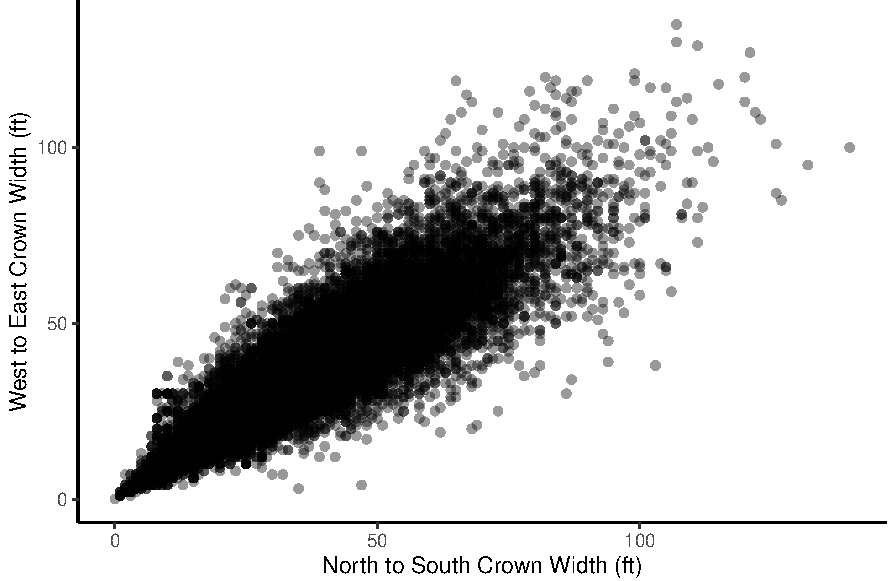
\includegraphics{thesis_files/figure-latex/crownWidth-1} 

}

\caption{Plot comparing North to South Crown Width (ft) to West to East Crown Width (ft). A tree with a higher north-south crown width has a higher west-east crown width, so without loss of generality the north-south crown width variable is used to filter the dataset for larger trees only.}\label{fig:crownWidth}
\end{figure}
Six tree types were determined to have large enough canopies on average and appear frequently enough to construct a training dataset with plenty of observations for each species of tree: Douglas-Fir, English Oak, Giant Sequoia, Maple, Western Redcedar. Table \ref{tab:pointsTable} provides the number of trees under each common name category. The largest group contains 6485 observations of Douglas-Fir trees, and the smallest group contains 135 observations of English Oak trees.
\begin{table}

\caption{\label{tab:pointsTable}Common tree names included in the tidy data and their total counts.}
\centering
\begin{tabular}[t]{l|r}
\hline
Tree Name & Tree Count\\
\hline
Douglas-Fir & 6485\\
\hline
Norway Maple & 1406\\
\hline
Western Redcedar & 652\\
\hline
Bigleaf Maple & 464\\
\hline
Giant Sequoia & 315\\
\hline
English Oak & 135\\
\hline
\end{tabular}
\end{table}
\hypertarget{creating-spatial-polygons}{%
\subsubsection{Creating Spatial Polygons}\label{creating-spatial-polygons}}

The training dataset was converted into shapefiles for each type of tree and exported into QGIS where polygons were manually drawn around 100 of the trees for each species. The point shapefile layers were displayed over the raster images downloaded from Planet.com in QGIS, which provided a guide point for locating individual trees. Then using QGIS's drawing tool, a polygon is carefully drawn around the tree canopy (see Figure \ref{fig:polyimage} and Figure \ref{fig:redcedar}). Most polygons turned out to be four to six-sided polygons to retain the general shape of the tree canopy. Trees polygons were only created if the outline of the tree canopy was clearly visible or surrounded by other trees of the same species in order to avoid including pixels from the wrong species in that polygon. Also, the shadows of the trees are visible in the raster images, so the polygons were drawn with the intention of not including the tree shadow. For the five different species of trees, at least 100 polygons were drawn around trees of that type, with each polygon containing at least 6 pixels and at most 20 pixels. The polygon shapefiles were then exported into RStudio where the rest of the analysis was conducted.
\begin{figure}

{\centering 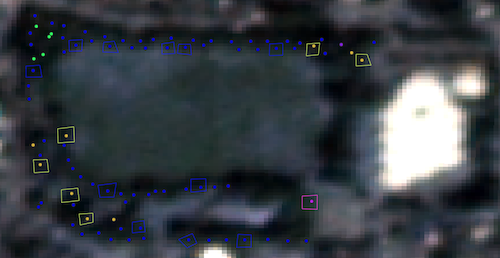
\includegraphics[width=0.5\linewidth]{figure/polyimage} 

}

\caption{Polygons drawn around different tree species: maples (blue), sequoias (yellow), redcedars (pink). Note there are no polygons around trees with canopies that overlap with canopies of different tree species, like douglas-firs (green), to avoid misclassifying pixels from different tree species.}\label{fig:polyimage}
\end{figure}
\begin{figure}

{\centering 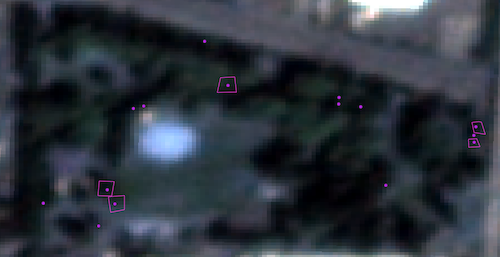
\includegraphics[width=0.5\linewidth]{figure/redcedar} 

}

\caption{Polygons drawn around redcedar trees}\label{fig:redcedar}
\end{figure}
\hypertarget{polygon-limitations}{%
\subsubsection{Polygon Limitations}\label{polygon-limitations}}

Ideally, the raster strips contain training trees of each species, and as a result, the polygons are evenly distributed across the raster strips, but due to limitations of our ground-level data this is not achievable. At a glace, each of the raster strips contain manually drawn polygons, so moving forward, it is assumed that there is equal variation across individual strips.

The polygons are drawn with the intention of outlining pixels for a known tree species so that the extracted pixels truly represent that species and so that there is a sufficient amount of pixels per species, however, limitations of the satellite images' resolution make some error inevitable. Many parks trees have canopies that overlap, which cause some polygons to contain pixels from trees of different species. Other pixel errors might come from including pixels that are cast in shadow by the polygon's training tree or by surrounding infrastructure. To avoid these errors, polygons with uncertain canopies are cross-checked with the satellite filter on Google Maps. For example, a point in QGIS that is indicated as a douglas-fir tree might appear as one tree on the low-resolution image from Planet.com, but a closer look at Google Maps shows that it is actually two trees in close proximity. Having low spatial resolution decreases the number of pixels available within a polygon, but that has to be balanced out with the need for a large number of pixels. With regards to the number of pixels per tree species, having around the same number of tree polygons per species results in differing amounts of pixels per species due to the different average sizes of tree canopies for different species. After drawing the images, the pixels totals per tree species is computed to ensure that the training pixels data contains at least 800 pixels per tree species.

\hypertarget{combining-ground-level-data-with-pixel-level-data}{%
\subsubsection{Combining Ground-level Data with Pixel-level Data}\label{combining-ground-level-data-with-pixel-level-data}}

The first spatial join in RStudio was conducted to match up each Spatial Polygon with a point in the training dataset. Then the raster images were loaded and joined with the polygons to extract the pixel values inside each polygon for all 4 bands (red, green, blue, infrared). Ultimately this turned into a pixel table with rows representing each pixel with its corresponding polygon, light reflection intensity values for all 4 bands, and the ground information about that tree. Table \ref{tab:pixelHead} displays the first few entries of the pixels dataset. Table \ref{tab:pixelCounts} contains the summary of the total number of pixels for each tree type.
\begin{table}

\caption{\label{tab:pixelHead}Variables and pixel values included in the pixels dataset}
\centering
\resizebox{\linewidth}{!}{
\begin{tabular}[t]{r|r|r|r|r|l|l|l|l|r|r|r|l|l|r}
\hline
ID & red & green & blue & ir & id\_type & Genus & Species & Cmmn\_Nm & Cr\_W\_NS & Cr\_W\_EW & Crw\_B\_H & Conditn & St\_Wdth & ndvi\\
\hline
43 & 4707 & 4125 & 3187 & 6627 & acpl & Acer & ACPL & Norway Maple & 28 & 28 & 8 & Fair & NA & 0.1694018\\
\hline
43 & 4384 & 3860 & 2864 & 7111 & acpl & Acer & ACPL & Norway Maple & 28 & 28 & 8 & Fair & NA & 0.2372336\\
\hline
43 & 4446 & 3803 & 2807 & 7443 & acpl & Acer & ACPL & Norway Maple & 28 & 28 & 8 & Fair & NA & 0.2520818\\
\hline
43 & 4619 & 3911 & 2859 & 7801 & acpl & Acer & ACPL & Norway Maple & 28 & 28 & 8 & Fair & NA & 0.2561997\\
\hline
43 & 4695 & 4060 & 3201 & 5996 & acpl & Acer & ACPL & Norway Maple & 28 & 28 & 8 & Fair & NA & 0.1216911\\
\hline
43 & 4344 & 3719 & 2728 & 6747 & acpl & Acer & ACPL & Norway Maple & 28 & 28 & 8 & Fair & NA & 0.2166622\\
\hline
\end{tabular}}
\end{table}
\begin{table}

\caption{\label{tab:pixelCounts}Number of pixels per tree type}
\centering
\begin{tabular}[t]{l|r}
\hline
Tree Name & Pixels Count\\
\hline
Bigleaf Maple & 885\\
\hline
Douglas-Fir & 1380\\
\hline
English Oak & 1025\\
\hline
Giant Sequoia & 1436\\
\hline
grass & 2923\\
\hline
Norway Maple & 2340\\
\hline
Western Redcedar & 1364\\
\hline
\end{tabular}
\end{table}
Figure \ref{fig:pixDensity} displays the range of reflection intensity pixel values per tree type. Each tree species has similar ranges of values over the red, green, blue, and infared bands. Of the species included in the training data, the Giant Sequoia trees appear to have higher density counts for the red, green, and blue bands.
\begin{figure}

{\centering 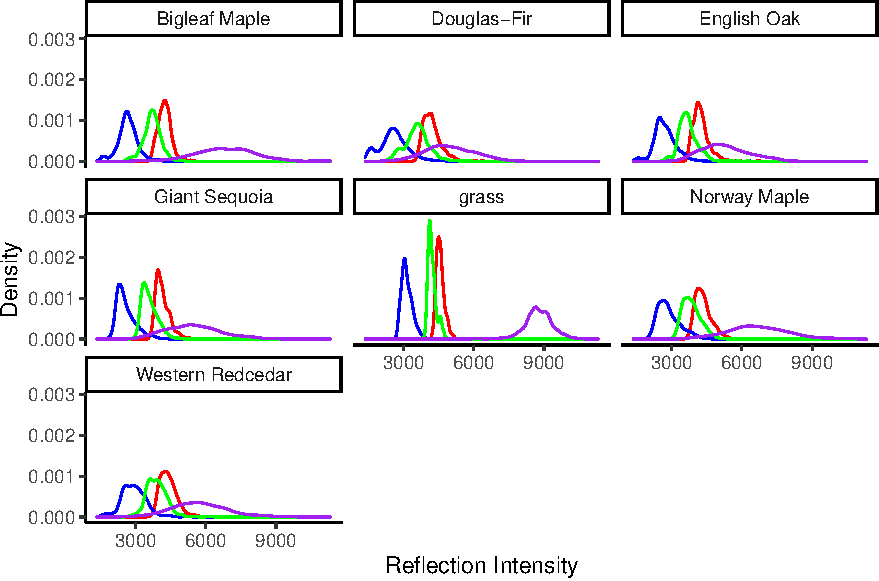
\includegraphics{thesis_files/figure-latex/pixDensity-1} 

}

\caption{ }\label{fig:pixDensity}
\end{figure}
--\textgreater{}

\hypertarget{methods}{%
\chapter{Methods}\label{methods}}

\hypertarget{current-methods}{%
\section{Current Methods}\label{current-methods}}

Since the Western redcedar decline is recent, there are currently no methods for identifying tree species like Western redcedars for the Pacific Northwest using satellite imaging. However, a similar study identifies tree species for a strip of land in California by combining ground-level data with satellite images (Fricker et al., 2019). Their methods involved drawing polygons around rastered images that are layered with ground data as explained in Chapter \ref{data}, but the pixels from the polygons are used to train a convolutional neural network (CNN) model instead of the random forests and support vector machines in this study. The CNN model was then evaluated with k-fold cross validation. CNN models are appropriate in a classification setting and when working with satellite images because they account for spatial relations, which is likely to appear in classifying tree species. This study follows the methods of preparing the data for modelling as well as the cross validation method to evaluate the performance of the random forests and support vector machines models. Random forests use random feature selections to create decision trees and increase the number of correctly classified observations. Random forests have the advantage of being simplier to train and still performs at a similar level as CNN models.

\hypertarget{training-models}{%
\section{Training Models}\label{training-models}}

To model the tree type of the pixels in raster image, a random forest model and a support vector machine model are trained using the pixels training data. To train these models, k-fold cross validation is used. The data gets split into \(k = 10\) folds and ten models are trained each time withholding one of the ten folds until the process goes through every fold. This process aids in understanding how the models will perform against data that has not been included in training the model.

The selected variables for training the models are the four bands (red, green, blue, infrared) and an NDVI variable, and the predictive variable is the tree species name. The \texttt{caret} package (Kuhn, 2020) in RStudio stands for classification and regression training, and it contains functions for facilitating the process of creating training models in R.

The \texttt{train} function from the \texttt{caret} package (Kuhn, 2020) with the specified \texttt{method\ =\ rf} option is used to train a random forest model on the training dataset to predict the tree species. The function takes parameters for data, the predictive variable, and the method of training the model. To perform k-fold cross validation, the \texttt{trainControl} function is used to create an object that tells the \texttt{train} function to perform cross validation 10 times with a different fold left out each time.

The \texttt{train} function also has the \texttt{method\ =\ svmLinear/svmRadial/svmPoly} option to train a support vector machine model on the training dataset to classify pixels into species of trees. This option also has parameter for cost, loss function, class weights, and normalized variables. For this project, three support vector machines were trained: linear, radial basis, and polynomial basis, and all three were specified to normalize the variables.

The models are saved to be used for later prediction over the entire region of Portland.

\hypertarget{preparing-raster-images}{%
\section{Preparing Raster Images}\label{preparing-raster-images}}

The training model has to be applied to the entire raster image to predict the location of Western redcedars, however, extracting all the pixels from raster images is a slow process. Filtering the rasters to keep vegetation and to recognize the difference between grass pixels and tree pixels alleviates the computational intensity of extracting all the pixels and improves the performance of the models.

\hypertarget{masking-vegetation}{%
\subsection{Masking Vegetation}\label{masking-vegetation}}

The satellite images in RStudio need to be masked to reduce the number of pixels that the model has to classify and prevent the chance of a non-vegetation surface being predicted as a tree. A common mask applied to raster images is a Normalized Difference Vegetation Index (NDVI) mask. This index is a measure of the greenness of a pixel, with higher values indicating vegetation and lower values indicating infertile areas such as a rock. The formula for NDVI is \(NDVI = \frac{NIR - Red}{NIR + Red}\). Figure \ref{fig:ndvival} displays the density of NDVI values over the raster images. To remove the pixels that are not vegetation, an NDVI threshold is determined to be 0.00 to create a mask dividing the pixels into vegetation (1) and non-vegetation (0). When the trained model is applied to the raster image, it is applied to the masked raster image that only keeps pixels with NDVI mask values of 1.
\begin{figure}

{\centering 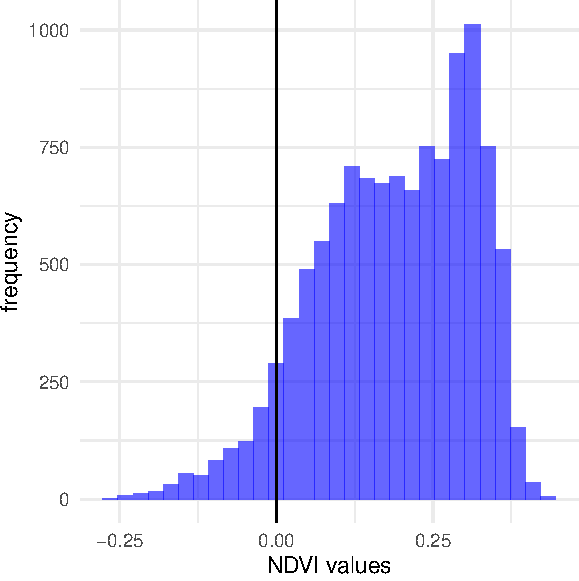
\includegraphics{thesis_files/figure-latex/ndvival-1} 

}

\caption{Normalized Difference Vegetation Index (NDVI) is a measure of the greenness of a pixel. The histogram displays the frequency of the tree pixels' NDVI values. A good threshold for masking out the nonvegetation pixels is an NDVI of 0.}\label{fig:ndvival}
\end{figure}
\hypertarget{masking-grass}{%
\subsection{Masking Grass}\label{masking-grass}}

A second mask is applied to the NDVI masked raster image to distinguish tree pixels from grass pixels. Inspired by previous research, a grass index was created by averaging the values of the four bands, \(GRASS = \frac{RED + BLUE + GREEN + NIR}{4}\) (Qian, Zhou, Nytch, Han, \& Li, 2020). Grass polygons were created in QGIS to add a grass attribute in the pixels dataset. Five fields of grass were outlined as polygons in QGIS. In RStudio, the pixels were extracted from the grass polygons for a total of 2,923 grass pixels. Figure \ref{fig:grassval} displays how the average band values for the grass pixels idffer from the other tree types average band values. Based on the figure, pixels in the raster image that have an average band value above 4900 are filtered out. Masking the grass pixels ensures that a field of grass will not be classified as a tree when applied to the entire raster image
\begin{figure}

{\centering 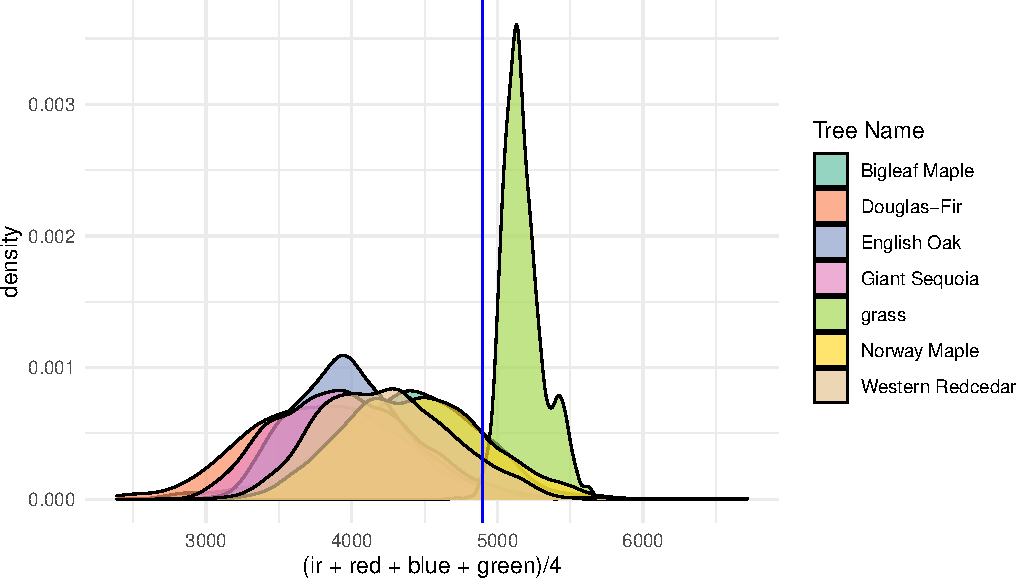
\includegraphics{thesis_files/figure-latex/grassval-1} 

}

\caption{grass mask}\label{fig:grassval}
\end{figure}
Figure \ref{fig:beforeaftermask} displays a raster strip with every pixel included (top), only the pixels with NDVI values above 0.00 (middle), and only pixels with NDVI values above 0.00 and average band values below 4900 (bottom). Ideally, the bottom image is left with only the tree pixels in the image.
\begin{figure}

{\centering 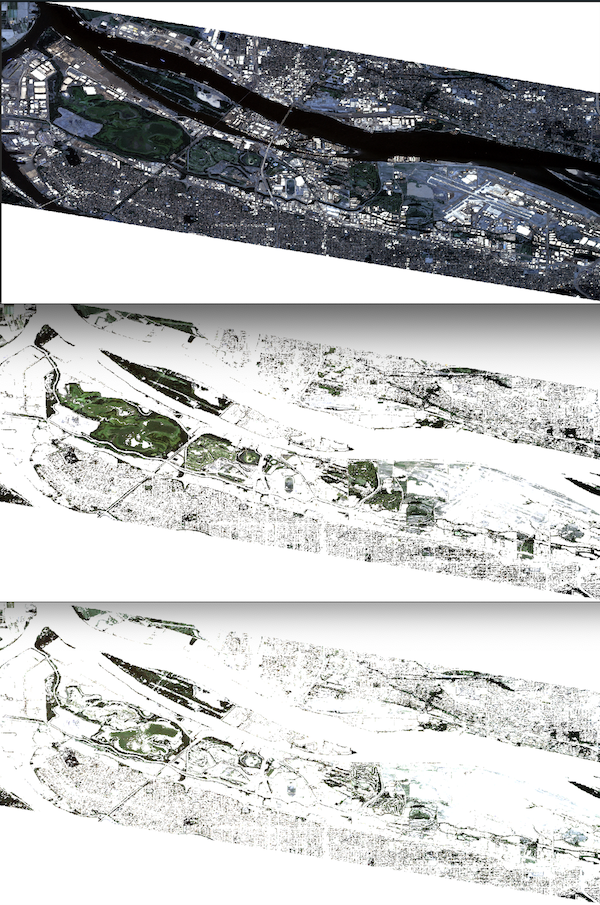
\includegraphics[width=0.4\linewidth]{figure/beforeaftermask} 

}

\caption{A raster strip with every pixel included (top), only the pixels with NDVI values above 0.00 (middle), and only pixels with NDVI values above 0.00 and average band values below 4900 (bottom)}\label{fig:beforeaftermask}
\end{figure}
\hypertarget{masking-limitations}{%
\subsection{Masking Limitations}\label{masking-limitations}}

The low resolution of the raster images cause shapes to appear blurry, and especially tree canopies that are close together appear as a single formation.

Masked raster images were compared in QGIS and, in general, the masks are successful in keeping the forest pixels while still removing building structures and roads. If a field of grass is a brownish color, it gets removed, but some greener fields are not masked out. The masks consistently remove river pixels but not lake pixels if the lake is a greenish color. For example, Smith Lake in North Portland is considered an urban wetland, which signifies a body of water with a lot of vegetation. From the perspective of a satellite, this looks like a field of grass. However, the average band pixel values are less than 4900, so they are not masked out by the final GRASS mask stage, and instead are treated as tree pixels in the model (see Figure \ref{fig:masklimit}).
\begin{figure}

{\centering 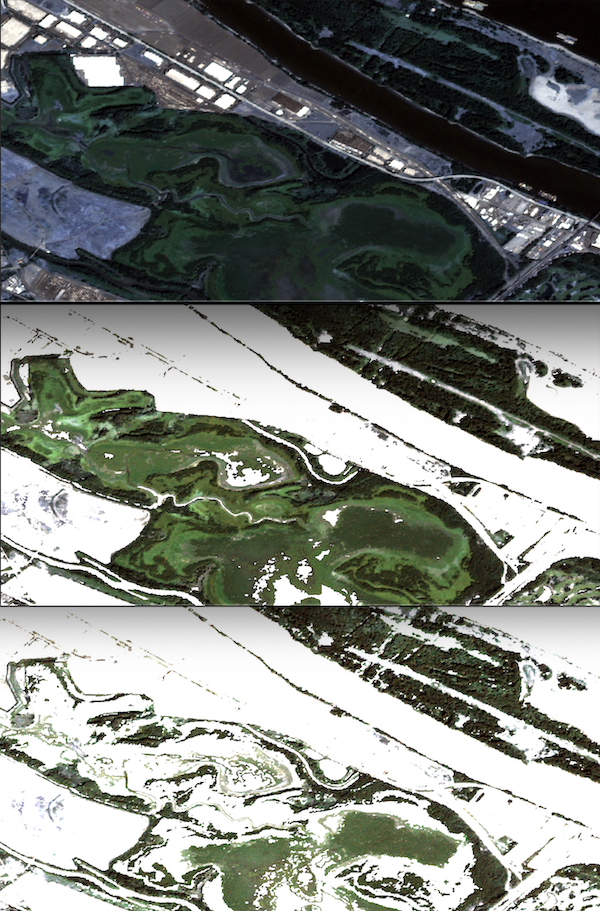
\includegraphics[width=0.4\linewidth]{figure/masklimit} 

}

\caption{Satellite view of Smith Lake (top), after NDVI mask applied (middle), and NDVI mask and GRASS mask applied (bottom). The final masked image still contains parts of the lake because the aquatic vegetation fits the pixel values descriptions set by the masks.}\label{fig:masklimit}
\end{figure}
\hypertarget{modelling-tree-species-in-portland}{%
\section{Modelling Tree Species in Portland}\label{modelling-tree-species-in-portland}}

After masking the raster images of the entire region of Portland, the pre-trained models are used to predict the tree species of individual pixels in the masked raster images. First the pixels are extracted from the raster and compiled into a dataset. Then the models are applied to predict the tree species per pixel in the dataset.

\hypertarget{conclusion}{%
\chapter*{Conclusion}\label{conclusion}}
\addcontentsline{toc}{chapter}{Conclusion}

If we don't want Conclusion to have a chapter number next to it, we can add the \texttt{\{-\}} attribute.

\textbf{More info}

And here's some other random info: the first paragraph after a chapter title or section head \emph{shouldn't be} indented, because indents are to tell the reader that you're starting a new paragraph. Since that's obvious after a chapter or section title, proper typesetting doesn't add an indent there.

\appendix

\hypertarget{the-first-appendix}{%
\chapter{The First Appendix}\label{the-first-appendix}}

This first appendix includes all of the R chunks of code that were hidden throughout the document (using the \texttt{include\ =\ FALSE} chunk tag) to help with readibility and/or setup.

\textbf{In the main Rmd file}
\begin{Shaded}
\begin{Highlighting}[]
\CommentTok{# This chunk ensures that the thesisdown package is}
\CommentTok{# installed and loaded. This thesisdown package includes}
\CommentTok{# the template files for the thesis.}
\ControlFlowTok{if}\NormalTok{(}\OperatorTok{!}\KeywordTok{require}\NormalTok{(devtools))}
  \KeywordTok{install.packages}\NormalTok{(}\StringTok{"devtools"}\NormalTok{, }\DataTypeTok{repos =} \StringTok{"http://cran.rstudio.com"}\NormalTok{)}
\ControlFlowTok{if}\NormalTok{(}\OperatorTok{!}\KeywordTok{require}\NormalTok{(thesisdown))}
\NormalTok{  devtools}\OperatorTok{::}\KeywordTok{install_github}\NormalTok{(}\StringTok{"ismayc/thesisdown"}\NormalTok{)}
\KeywordTok{library}\NormalTok{(thesisdown)}
\end{Highlighting}
\end{Shaded}
\textbf{In Chapter \ref{ref-labels}:}
\begin{Shaded}
\begin{Highlighting}[]
\CommentTok{# This chunk ensures that the thesisdown package is}
\CommentTok{# installed and loaded. This thesisdown package includes}
\CommentTok{# the template files for the thesis and also two functions}
\CommentTok{# used for labeling and referencing}
\ControlFlowTok{if}\NormalTok{ (}\OperatorTok{!}\KeywordTok{require}\NormalTok{(remotes)) \{}
  \ControlFlowTok{if}\NormalTok{ (params}\OperatorTok{$}\StringTok{`}\DataTypeTok{Install needed packages for \{thesisdown\}}\StringTok{`}\NormalTok{) \{}
    \KeywordTok{install.packages}\NormalTok{(}\StringTok{"remotes"}\NormalTok{, }\DataTypeTok{repos =} \StringTok{"https://cran.rstudio.com"}\NormalTok{)}
\NormalTok{  \} }\ControlFlowTok{else}\NormalTok{ \{}
    \KeywordTok{stop}\NormalTok{(}
      \KeywordTok{paste}\NormalTok{(}
        \StringTok{'You need to run install.packages("remotes")'}\NormalTok{,}
        \StringTok{"first in the Console."}
\NormalTok{      )}
\NormalTok{    )}
\NormalTok{  \}}
\NormalTok{\}}
\ControlFlowTok{if}\NormalTok{ (}\OperatorTok{!}\KeywordTok{require}\NormalTok{(dplyr)) \{}
  \ControlFlowTok{if}\NormalTok{ (params}\OperatorTok{$}\StringTok{`}\DataTypeTok{Install needed packages for \{thesisdown\}}\StringTok{`}\NormalTok{) \{}
    \KeywordTok{install.packages}\NormalTok{(}\StringTok{"dplyr"}\NormalTok{, }\DataTypeTok{repos =} \StringTok{"https://cran.rstudio.com"}\NormalTok{)}
\NormalTok{  \} }\ControlFlowTok{else}\NormalTok{ \{}
    \KeywordTok{stop}\NormalTok{(}
      \KeywordTok{paste}\NormalTok{(}
        \StringTok{'You need to run install.packages("dplyr")'}\NormalTok{,}
        \StringTok{"first in the Console."}
\NormalTok{      )}
\NormalTok{    )}
\NormalTok{  \}}
\NormalTok{\}}
\ControlFlowTok{if}\NormalTok{ (}\OperatorTok{!}\KeywordTok{require}\NormalTok{(ggplot2)) \{}
  \ControlFlowTok{if}\NormalTok{ (params}\OperatorTok{$}\StringTok{`}\DataTypeTok{Install needed packages for \{thesisdown\}}\StringTok{`}\NormalTok{) \{}
    \KeywordTok{install.packages}\NormalTok{(}\StringTok{"ggplot2"}\NormalTok{, }\DataTypeTok{repos =} \StringTok{"https://cran.rstudio.com"}\NormalTok{)}
\NormalTok{  \} }\ControlFlowTok{else}\NormalTok{ \{}
    \KeywordTok{stop}\NormalTok{(}
      \KeywordTok{paste}\NormalTok{(}
        \StringTok{'You need to run install.packages("ggplot2")'}\NormalTok{,}
        \StringTok{"first in the Console."}
\NormalTok{      )}
\NormalTok{    )}
\NormalTok{  \}}
\NormalTok{\}}
\ControlFlowTok{if}\NormalTok{ (}\OperatorTok{!}\KeywordTok{require}\NormalTok{(bookdown)) \{}
  \ControlFlowTok{if}\NormalTok{ (params}\OperatorTok{$}\StringTok{`}\DataTypeTok{Install needed packages for \{thesisdown\}}\StringTok{`}\NormalTok{) \{}
    \KeywordTok{install.packages}\NormalTok{(}\StringTok{"bookdown"}\NormalTok{, }\DataTypeTok{repos =} \StringTok{"https://cran.rstudio.com"}\NormalTok{)}
\NormalTok{  \} }\ControlFlowTok{else}\NormalTok{ \{}
    \KeywordTok{stop}\NormalTok{(}
      \KeywordTok{paste}\NormalTok{(}
        \StringTok{'You need to run install.packages("bookdown")'}\NormalTok{,}
        \StringTok{"first in the Console."}
\NormalTok{      )}
\NormalTok{    )}
\NormalTok{  \}}
\NormalTok{\}}
\ControlFlowTok{if}\NormalTok{ (}\OperatorTok{!}\KeywordTok{require}\NormalTok{(thesisdown)) \{}
  \ControlFlowTok{if}\NormalTok{ (params}\OperatorTok{$}\StringTok{`}\DataTypeTok{Install needed packages for \{thesisdown\}}\StringTok{`}\NormalTok{) \{}
\NormalTok{    remotes}\OperatorTok{::}\KeywordTok{install_github}\NormalTok{(}\StringTok{"ismayc/thesisdown"}\NormalTok{)}
\NormalTok{  \} }\ControlFlowTok{else}\NormalTok{ \{}
    \KeywordTok{stop}\NormalTok{(}
      \KeywordTok{paste}\NormalTok{(}
        \StringTok{"You need to run"}\NormalTok{,}
        \StringTok{'remotes::install_github("ismayc/thesisdown")'}\NormalTok{,}
        \StringTok{"first in the Console."}
\NormalTok{      )}
\NormalTok{    )}
\NormalTok{  \}}
\NormalTok{\}}
\KeywordTok{library}\NormalTok{(thesisdown)}
\KeywordTok{library}\NormalTok{(dplyr)}
\KeywordTok{library}\NormalTok{(ggplot2)}
\KeywordTok{library}\NormalTok{(knitr)}
\NormalTok{flights <-}\StringTok{ }\KeywordTok{read.csv}\NormalTok{(}\StringTok{"data/flights.csv"}\NormalTok{, }\DataTypeTok{stringsAsFactors =} \OtherTok{FALSE}\NormalTok{)}
\end{Highlighting}
\end{Shaded}
\hypertarget{the-second-appendix-for-fun}{%
\chapter{The Second Appendix, for Fun}\label{the-second-appendix-for-fun}}

\backmatter

\hypertarget{references}{%
\chapter*{References}\label{references}}
\addcontentsline{toc}{chapter}{References}

\markboth{References}{References}

\noindent

\setlength{\parindent}{-0.20in}
\setlength{\leftskip}{0.20in}
\setlength{\parskip}{8pt}

\hypertarget{refs}{}
\leavevmode\hypertarget{ref-castelluccio_land_2015}{}%
Castelluccio, M., Poggi, G., Sansone, C., \& Verdoliva, L. (2015). Land Use Classification in Remote Sensing Images by Convolutional Neural Networks. \emph{arXiv:1508.00092 {[}Cs{]}}. Retrieved from \url{http://arxiv.org/abs/1508.00092}

\leavevmode\hypertarget{ref-fricker_convolutional_2019}{}%
Fricker, G. A., Ventura, J. D., Wolf, J. A., North, M. P., Davis, F. W., \& Franklin, J. (2019). A Convolutional Neural Network Classifier Identifies Tree Species in Mixed-Conifer Forest from Hyperspectral Imagery. \emph{Remote Sensing}, \emph{11}(19), 2326. \url{http://doi.org/10.3390/rs11192326}

\leavevmode\hypertarget{ref-caret}{}%
Kuhn, M. (2020). \emph{Caret: Classification and regression training}. Retrieved from \url{https://CRAN.R-project.org/package=caret}

\leavevmode\hypertarget{ref-peterson_western_nodate}{}%
Peterson, J. S. (n.d.). WESTERN RED CEDAR, 3.

\leavevmode\hypertarget{ref-qian_new_2020}{}%
Qian, Y., Zhou, W., Nytch, C. J., Han, L., \& Li, Z. (2020). A new index to differentiate tree and grass based on high resolution image and object-based methods. \emph{Urban Forestry \& Urban Greening}, \emph{53}, 126661. \url{http://doi.org/10.1016/j.ufug.2020.126661}

\leavevmode\hypertarget{ref-noauthor_western_nodate-1}{}%
Western red cedar. (n.d.). Retrieved from \url{https://www.oregonencyclopedia.org/articles/western_red_cedar/\#.YB7fUy1h1N0}

\leavevmode\hypertarget{ref-noauthor_western_nodate}{}%
Western redcedar Dieback. (n.d.). \emph{PPO Home}. Retrieved from \url{https://ppo.puyallup.wsu.edu/plant-health-concerns/redcedar/}


% Index?

\end{document}
